\PassOptionsToPackage{unicode=true}{hyperref} % options for packages loaded elsewhere
\PassOptionsToPackage{hyphens}{url}
\documentclass[12pt,ignorenonframetext,aspectratio=169]{beamer}
\IfFileExists{pgfpages.sty}{\usepackage{pgfpages}}{}
\setbeamertemplate{caption}[numbered]
\setbeamertemplate{caption label separator}{: }
\setbeamercolor{caption name}{fg=normal text.fg}
\beamertemplatenavigationsymbolsempty
\usepackage{lmodern}
\usepackage{amssymb}
\usepackage{amsmath}
\usepackage{ifxetex,ifluatex}
\usepackage{fixltx2e} % provides \textsubscript
\ifnum 0\ifxetex 1\fi\ifluatex 1\fi=0 % if pdftex
  \usepackage[T1]{fontenc}
  \usepackage[utf8]{inputenc}
\else % if luatex or xelatex
  \ifxetex
    \usepackage{mathspec}
  \else
    \usepackage{fontspec}
\fi
\defaultfontfeatures{Ligatures=TeX,Scale=MatchLowercase}






%
\fi

  \usetheme[]{iqss}






% use upquote if available, for straight quotes in verbatim environments
\IfFileExists{upquote.sty}{\usepackage{upquote}}{}
% use microtype if available
\IfFileExists{microtype.sty}{%
  \usepackage{microtype}
  \UseMicrotypeSet[protrusion]{basicmath} % disable protrusion for tt fonts
}{}


\newif\ifbibliography


\hypersetup{
      pdftitle={Value chain analysis: Concept, mapping and approaches},
        pdfauthor={Deependra Dhakal},
          pdfborder={0 0 0},
    breaklinks=true}
%\urlstyle{same}  % Use monospace font for urls







% Prevent slide breaks in the middle of a paragraph:
\widowpenalties 1 10000
\raggedbottom

  \AtBeginPart{
    \let\insertpartnumber\relax
    \let\partname\relax
    \frame{\partpage}
  }
  \AtBeginSection{
    \ifbibliography
    \else
      \let\insertsectionnumber\relax
      \let\sectionname\relax
      \frame{\sectionpage}
    \fi
  }
  \AtBeginSubsection{
    \let\insertsubsectionnumber\relax
    \let\subsectionname\relax
    \frame{\subsectionpage}
  }



\setlength{\parindent}{0pt}
\setlength{\parskip}{6pt plus 2pt minus 1pt}
\setlength{\emergencystretch}{3em}  % prevent overfull lines
\providecommand{\tightlist}{%
  \setlength{\itemsep}{0pt}\setlength{\parskip}{0pt}}

  \setcounter{secnumdepth}{0}


  \usepackage{booktabs}
  \usepackage{longtable}
  \usepackage{emptypage}
  \usepackage{array}
  \usepackage{multirow}
  \usepackage{wrapfig}
  \usepackage{float}
  \usepackage{colortbl}
  \usepackage{pdflscape}
  \usepackage{tabu}
  \usepackage{threeparttable}
  \usepackage{threeparttablex}
  \usepackage[normalem]{ulem}
  \usepackage{rotating}
  \usepackage{makecell}
  \usepackage{xcolor}
  \usepackage{tikz} % required for image opacity change
  \usepackage[absolute,overlay]{textpos} % for text formatting
  \usepackage[utf8]{inputenc}
  \usetikzlibrary{mindmap,arrows,shapes,positioning,shadows,trees}
  \usepackage[skip=2pt]{caption}

  % this font option is amenable for beamer
  \setbeamerfont{caption}{size=\tiny}


%% IQSS overrides
\iqsssectiontitle{Outline}

\AtBeginSection[]{
  \title{\insertsectionhead}
  {
    \definecolor{white}{rgb}{0.776,0.357,0.157}
    \definecolor{iqss@orange}{rgb}{1,1,1}
    \ifnum \insertmainframenumber > \insertframenumber
    \frame{
      \frametitle{\iqsssectiontitleheader}
      \tableofcontents[currentsection]
    }
    \else
    \frame{
      \frametitle{Backup Slides}
      \tableofcontents[sectionstyle=shaded/shaded,subsectionstyle=shaded/shaded/shaded]
    }
    \fi
  }
}

\AtBeginSubsection[]{}

%%


  \title[]{Value chain analysis: Concept, mapping and approaches}



  \author[
        Deependra Dhakal
    ]{Deependra Dhakal}

  \institute[
    ]{
    GAASC, Baitadi \and Tribhuwan University
    }

\date[
      \today
  ]{
      \today
        }

\begin{document}

% Hide progress bar and footline on titlepage
  \begin{frame}[plain]
  \titlepage
  \end{frame}



\hypertarget{value-chain}{%
\section{Value chain}\label{value-chain}}

\begin{frame}{Introduction}
\protect\hypertarget{introduction}{}
\begin{itemize}
\tightlist
\item
  Porter (1985) defined value chain is a chain of activities. Products
  pass through all activities of the chain in order and at each activity
  the product gains some value.
\item
  The value chain categorizes the generic value adding activities of an
  organization.
\item
  The ``primary activities'' include inbound logistics, operation
  (production), outbound logistics, sales and marketing, and service
  (maintenance).
\item
  The ``support activities'' include administrative infrastructure
  management, human resource management, research and development, and
  procurement.
\item
  The costs and value drivers are identified for each value activity.
  The value chain framework quickly makes its way to the forefront of
  management as a powerful analysis tool for strategic planning.
\item
  Its ultimate goal is to maximize value creation while minimizing cost.
\end{itemize}
\end{frame}

\begin{frame}{Mapping}
\protect\hypertarget{mapping}{}
\begin{itemize}
\tightlist
\item
  A value chain map graphically illustrates all of the components, and
  relationships between them, of the selected value chain.
\item
  It is a visual tool that helps us understand how a particular industry
  works.
\item
  Value chain maps demonstrate how a product in an industry moves from
  raw material through production, processing, and other steps, until it
  eventually winds up with the consumer.
\item
  The map highlights the range of activities that occur within the value
  chain.
\item
  The map will also outline transformation steps or functions, actors,
  relationships, and support services. The level of detail in a value
  chain map can vary, ranging from noting the basic essentials to highly
  comprehensive components.
\end{itemize}
\end{frame}

\begin{frame}{Mapping procedure}
\protect\hypertarget{mapping-procedure}{}
\begin{enumerate}
\tightlist
\item
  Collate market research
\item
  Write out each step in the transformation process
\item
  Identify the various end markets (consumers)
\item
  Identify the different actors
\item
  Depicting relationships (Arrow diagram)
\item
  Representing support services (Microfinance, Government extension and
  other serice, NGOs, Vale chain actors)
\item
  Add any additional overlays
\item
  Add gender dimension
\item
  Conduct additional market research and finalize
\end{enumerate}
\end{frame}

\begin{frame}{Value chain map: Example}
\protect\hypertarget{value-chain-map-example}{}
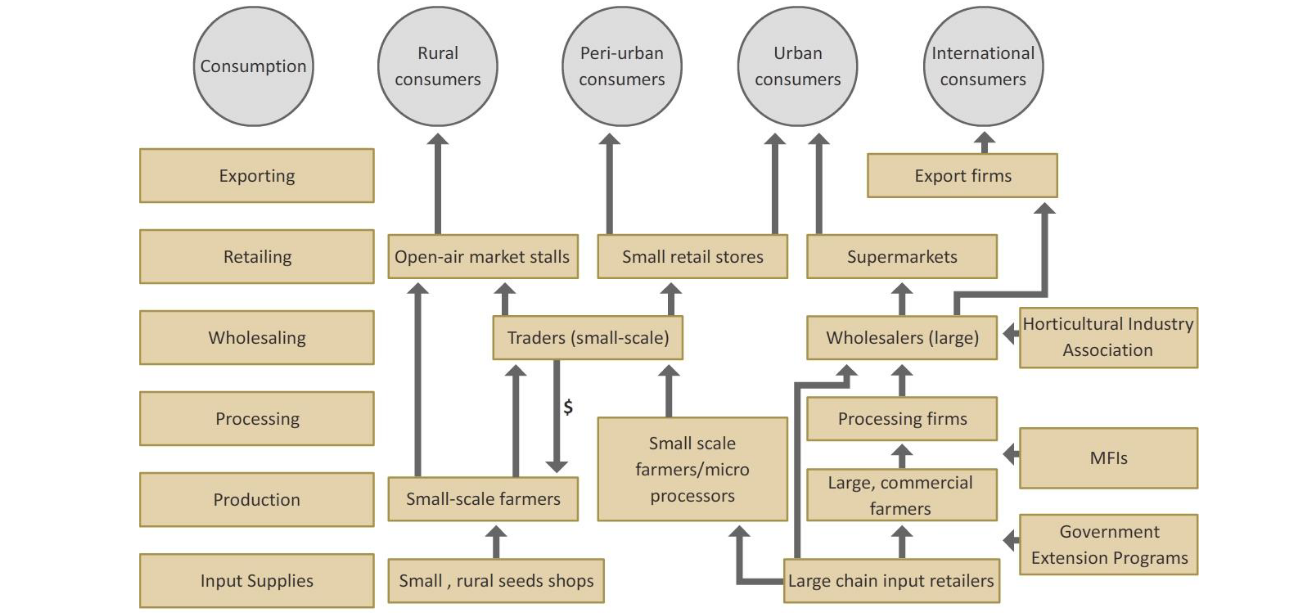
\includegraphics[width=0.85\linewidth]{./figs/value_chain_map}
\end{frame}

\hypertarget{porters-value-chain-analysis-approach}{%
\section{Porter's value chain analysis:
Approach}\label{porters-value-chain-analysis-approach}}

\begin{frame}{Porter's value chain analysis: Approach}
\begin{itemize}
\tightlist
\item
  Harvard Business School professor, Michael Porter, introduced a simple
  value chain model in his book, ``Competitive Advantage''. He developed
  the steps to perform a value chain analysis and split business
  activities into two categories: primary and support.
\end{itemize}

\begin{enumerate}
\tightlist
\item
  Determine the business' primary and support activities.
\end{enumerate}

Together, the primary and support activities make up the value chain.
And they include each action required in the development of a product or
service, from raw material to final product.
\end{frame}

\begin{frame}{}
\protect\hypertarget{section}{}
\begin{enumerate}
\setcounter{enumi}{1}
\tightlist
\item
  Analyze the value and cost of the activities.
\end{enumerate}

The team tasked with creating the value chain analysis should brainstorm
ways each activity provides value to customers and the business as a
whole. Compare the activity to the competitive advantage you're trying
to achieve (cost leadership or differentiation) and see if it supports
the goal.

After the value analysis is complete, take a look at the cost of the
activities. Is the activity labor intensive? How much does X raw
material cost? Asking questions similar to these will help identify
which activities are cost-effective and which are not. This where areas
for improvement can be identified.
\end{frame}

\begin{frame}{}
\protect\hypertarget{section-1}{}
\begin{enumerate}
\setcounter{enumi}{2}
\tightlist
\item
  Identify opportunities to gain a competitive advantage.
\end{enumerate}

Once the value chain analysis is complete, the primary stakeholders in
the business can see an overview of where the business is excelling and
where improvements can be made operationally.

Begin with the improvements that take minor changes and provide
high-impact results. After the easy wins are identified and actioned,
you and your team can tackle the bigger challenges that might be
hindering efficiency.

The value chain analysis gives businesses a clear idea of how to adjust
their actions and processes to provide the most value to their target
market and increase profit margins for the company.
\end{frame}




\end{document}
